\documentclass[a4paper,12pt,openany]{book}
\usepackage[T1]{fontenc}
\usepackage[utf8]{inputenc}
\usepackage{lmodern}
\usepackage{hyperref}
\usepackage{graphicx}
\usepackage{amsmath}
\graphicspath{ {images/} }
\usepackage[english]{babel}

\makeatletter
\renewcommand{\@chapapp}{}% Not necessary...
\newenvironment{chapquote}[2][2em]
  {\setlength{\@tempdima}{#1}%
   \def\chapquote@author{#2}%
   \parshape 1 \@tempdima \dimexpr\textwidth-2\@tempdima\relax%
   \itshape}
  {\par\normalfont\hfill--\ \chapquote@author\hspace*{\@tempdima}\par\bigskip}
\makeatother


% Book's title and subtitle
\title{\Huge \textbf{EVM Design}}\\ 
% Author
\author{\textsc{Deepanshu Jindal}}\\

\begin{document}

\frontmatter
\maketitle

\tableofcontents

\mainmatter

%%%%%%%%%%%
% Preface %
%%%%%%%%%%%
\chapter*{Preface}
This is a document which details the features of an ideal EVM and discusses the problems with the current EVM design in the country. Finally it looks upon a possible design of EVM which attempts to meet the features detailed in the first section.
\\


\chapter{What we expect from EVM}

\section{Coercion freedom}
We want the EVM to protect the voter's Right to Choice. We wish to ensure that the voter cannot be coerced by anybody to change his voting choice in an unfair way.
\\
This is closely tied to secrecy of vote as coercion freedom also means that nobody can determine with certainty to whom the voter voted by use of coercion.

\section{Secrecy}
Secrecy that if the voter doesn't want to disclose to whom he/she voted, then it should not be possible for anyone to determine with certainty that who the voter voted for.

\section{Anonymity}
The identity of the voter should be protected in all circumstances. Nobody should be able to identify a voter from the data of voting.

\section{Non-repudiation}
Nonrepudiation is the assurance that someone cannot deny something. Typically, nonrepudiation refers to the ability to ensure that a party to a contract or a communication cannot deny the authenticity of their signature on a document or the sending of a message that they originated. 
\\
In the context of voting it means that a voter cannot challenge that his vote was registered for a party different from whom he/she voted for.

\section{Verifiability}
Voter should be able to verify that his/her vote is counted towards the party he/she has voted for.\\
It should be possible to easily verify that the EVM is not tampered with. The authenticity of both hardware and the software of the EVM should be provable.

\section{Cryptosecure}
The data stored in EVM should be encrypted and cryptographically secure, so that any unauthorised third party cannot access it or tamper with it.

\section{Auditable}
It should be provable that the EVM works without any bias. There should be a proof of correctness of the entire process of voting. It should be possible to audit the process of voting at any stage and detect discrepancies if any.

\section{Self-certifiability}
The hardware and software should be self certifiable and tamper detection should be possible if one of them is compromised.

\section{Protection from information leakage}
The data stored inside the EVM should be protected from any kind of leakages. No third party should be able to access any sort of data from EVM during the process of voting and counting.

\newpage
\section{Constraints under which EVM are required to work}

\begin{itemize}
\item Cost effectiveness
\item Lack of electricity in remote areas
\item Illiteracy and unfamiliarity towards technology amongst population enforces adoption of simplistic designs
\item Booth capture
\end{itemize}

\chapter{The current design}
Elections in India are conducted almost exclusively using electronic voting machines developed over
the past two decades by a pair of government-owned companies. These devices, known in India as EVMs,
have been praised for their simple design, ease of use, and reliability, but recently they have also been
criticized following widespread reports of election irregularities.

\section{Operations and Procedure}
\begin{figure}[!h]
\centering
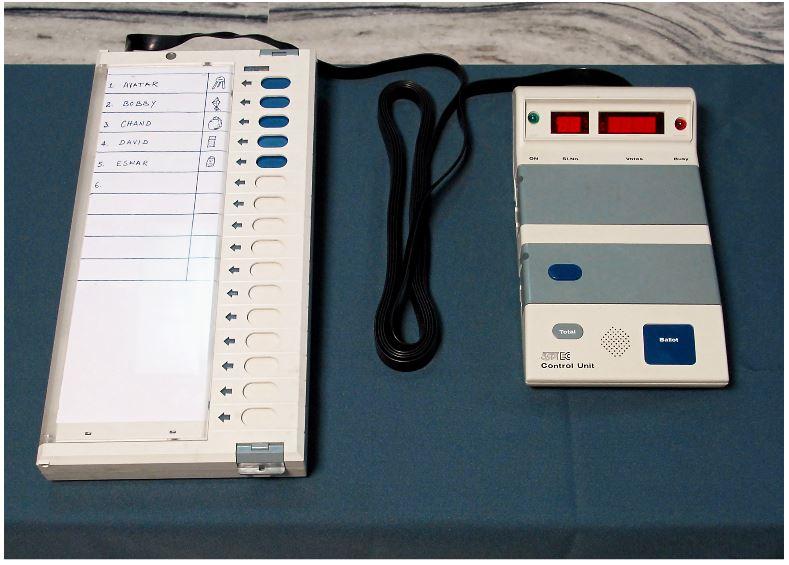
\includegraphics[scale=0.5]{EVM_with_Control_Unit.JPG}
\caption{The ballot and the control unit of EVM}
\end{figure}
\newpage
EVM consisted of two main components : Ballot unit and Control Unit.
Control Unit is used by poll
workers, which stores and accumulates votes.
Ballot Unit
is located in the election booth, which is
used by voters. These units are connected by a 5 m cable, which has one end permanently fixed to the ballot
unit.


The ballot unit has 16 candidate buttons. If any are unused, they are covered with a plastic masking tab
inside the unit. When there are more than 16 candidates, an additional ballot unit can be connected to a port on
the underside of the first ballot unit. Up to four ballot units can be chained together in this way, for a maximum
of 64 candidates.\\

Recently, a new unit called VVPAT was added to EVM to improve verifiability. Voter Verifiable Paper Audit Trail (VVPAT) or Verifiable Paper Record (VPR) is a method of providing feedback to voters using a ballotless voting system. A VVPAT is intended as an independent verification system for voting machines designed to allow voters to verify that their vote was cast correctly, to detect possible election fraud or malfunction, and to provide a means to audit the stored electronic results.
\newpage
\begin{figure}[!hb]
\centering
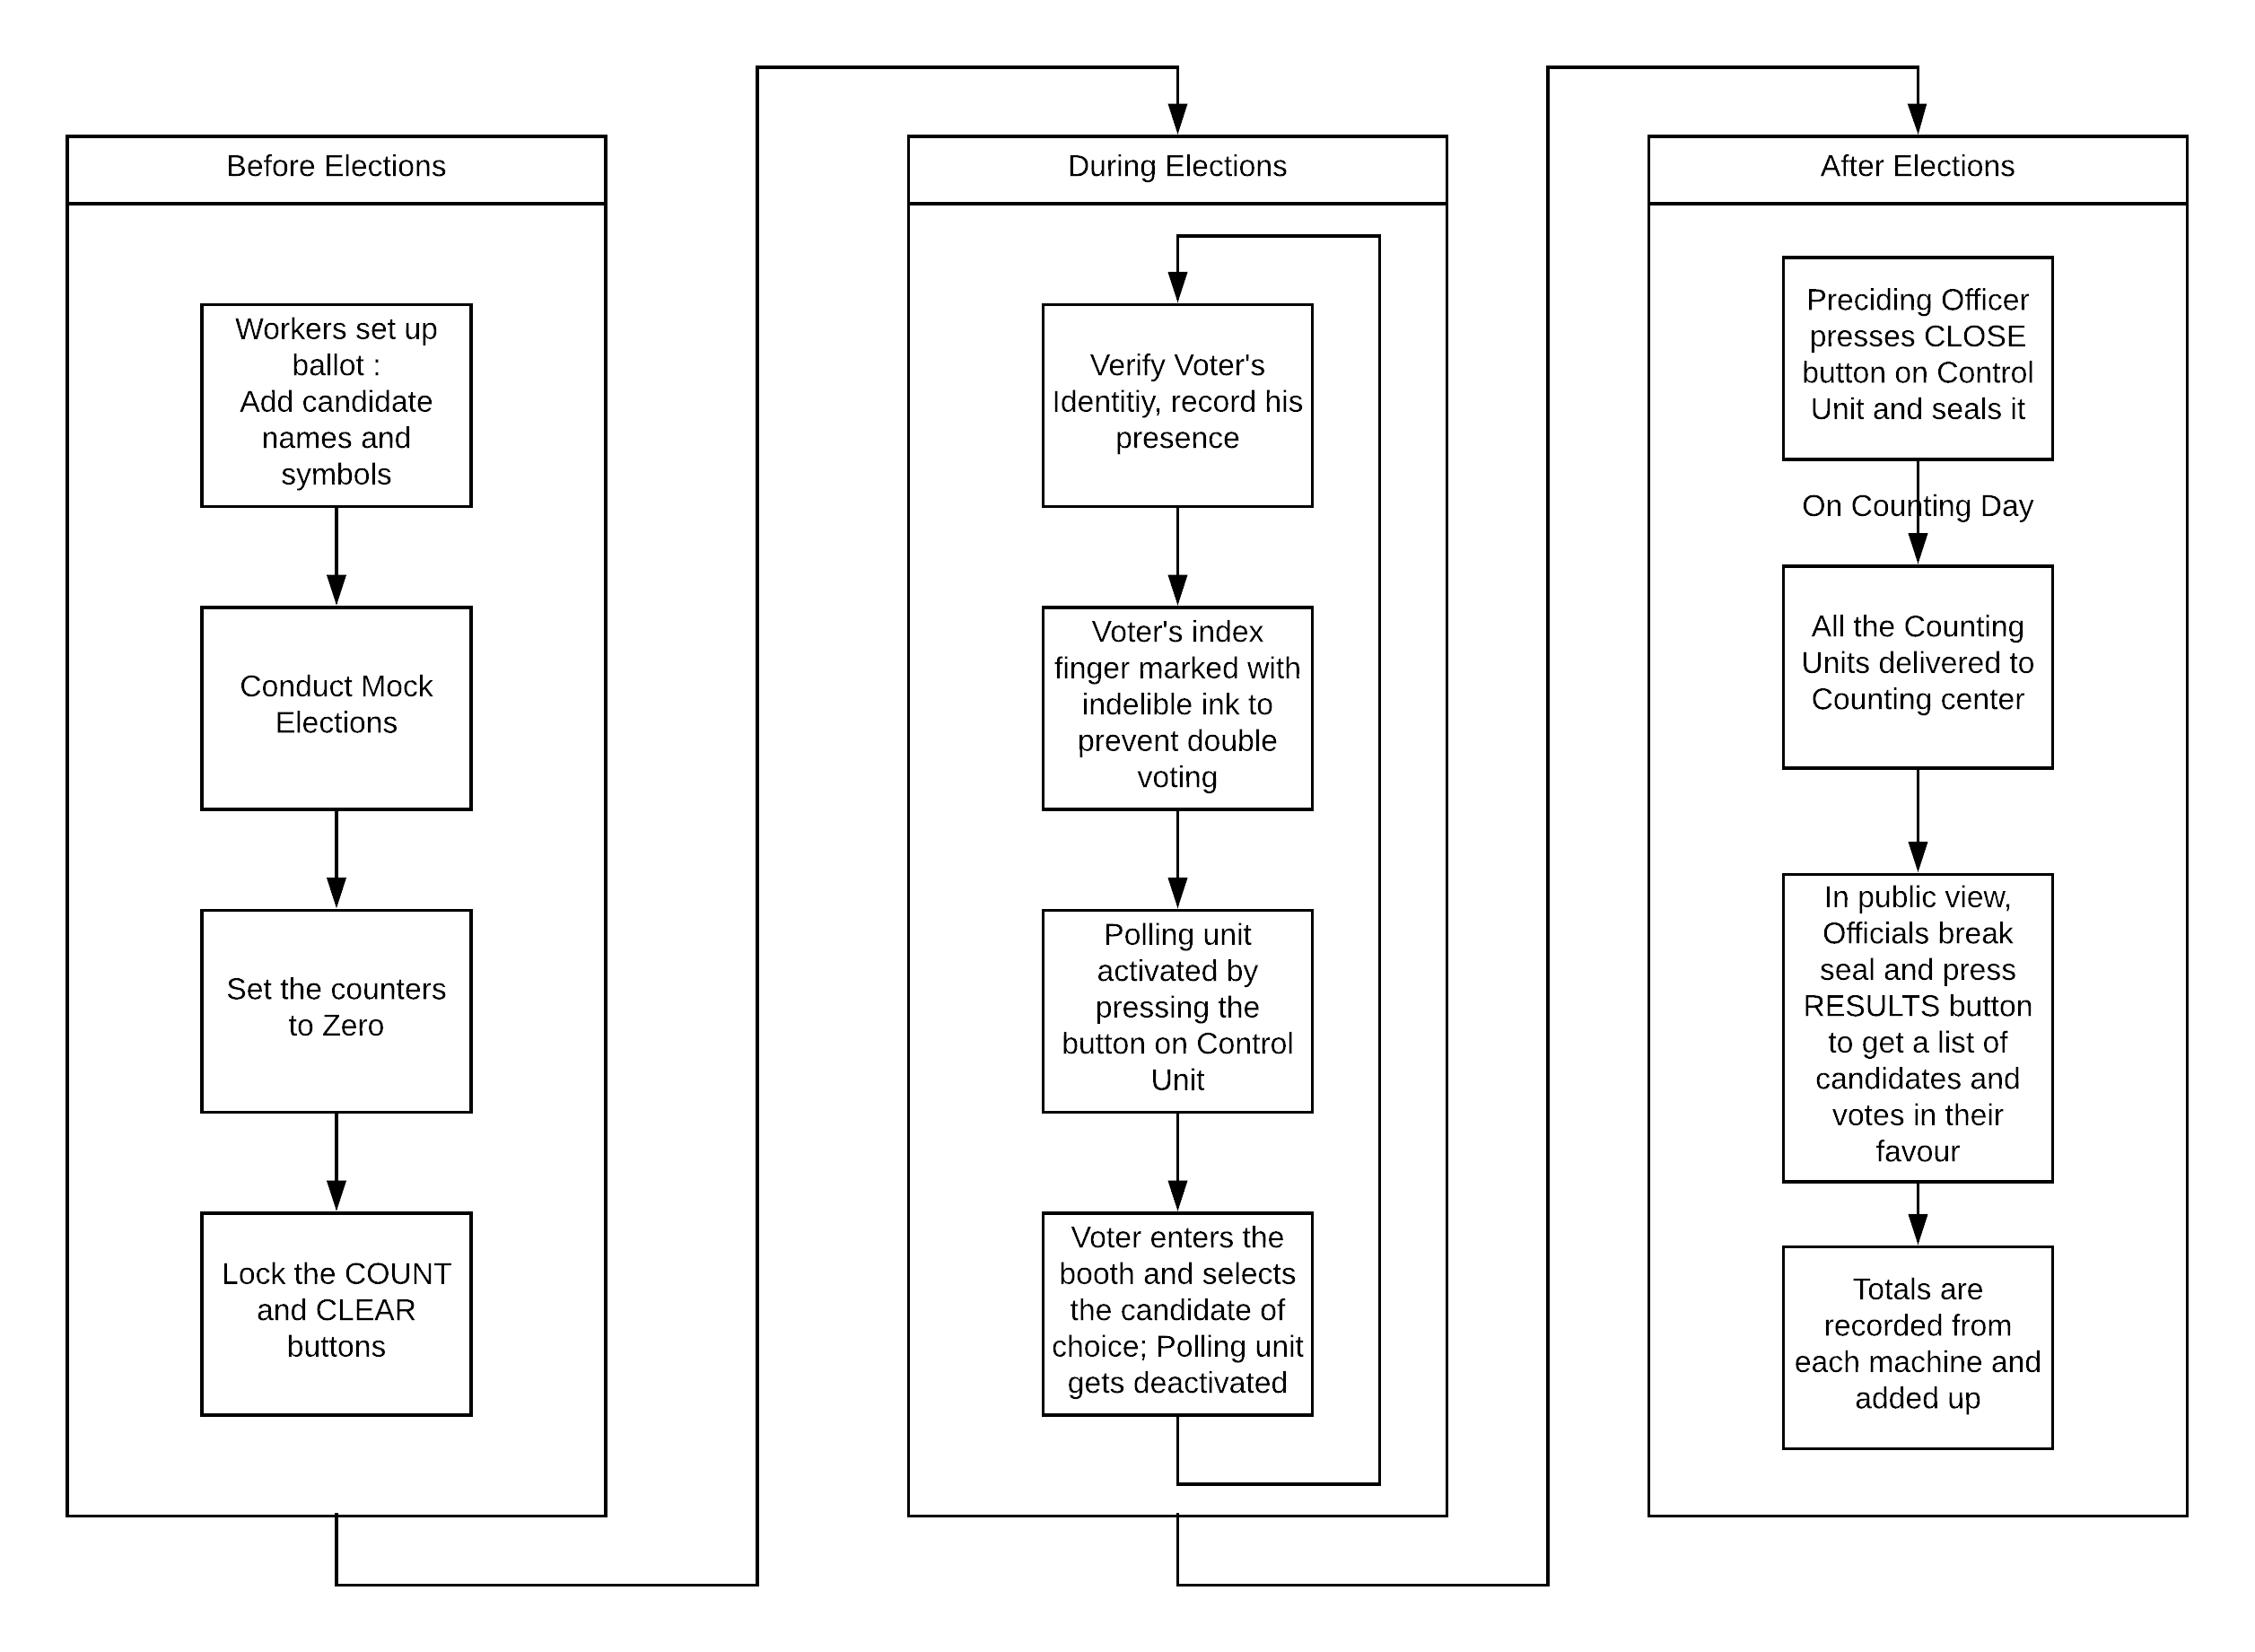
\includegraphics[scale=0.2]{FlowCurrent.PNG}
\caption{The flow diagram of electoral voting process}
\end{figure}
\newpage
\section{Issues with the design}
EVMs currently in use have a simplistic hardware design with software stored on ROM in order to prevent electrical reprogramming of software. However, even this simplistic device has certain vulnerabilities that can be exploited. Also the current design fails to ensure many of the features of the ideal EVM.

\begin{itemize}
\item \textbf{Lack of encryption} - The data is stored over the EVM in plain text format which makes it vulnerable to data leaks and placement of doppelganger components at the time of assembly. If the attacker gets access to data then he can simply read it off any bits to ASCII converter. This compromises properties of anonymity and secrecy.

\item \textbf{Oversimplicity} : The oversimplicity of design is itself a problem. Such simple designs means that certain defence mechanism cannot be placed and the tampering is easier.

\item \textbf{Multiple units} : Use of multiple units means greater chances of tampering. The link between control unit and the polling unit is an essentially critical link that is highly vulnerable to data leaks.

\item \textbf{Lack of verifiability} : Current EVM designs only provides namesake verifiability both about the state of authenticity and the casting of vote by the voter.

\item \textbf{Possibility of tampering before counting} : When the machines are sealed or unsealed before the counting process there are possibilities of tampering with EVM displays since votes are merely counted by reading off the display and registering them to the tally manually.

\item \textbf{Data Loss} : The data stored on Control units is vulnerable to physical or electromagnetic damage during storage. It is also vulnerable to physical damage by political party workers during the time of voting in case of booth capture. This puts at stake all the votes stored in the control unit.
\end{itemize}

\chapter{An attempt towards a new design}
The EVM that I propose tries to capture the maximal set of expectations from an ideal EVM and uses the shortcomings in current EVM design as cue points for further development.
\section{Walkthrough of features and the process}
\subsection{Authentication}
Authentication of voter incorporates two level of authentication.
Primary authentication happens through the existing procedure of authentication of identification documents by the polling officer. 

On successful primary authentication, the polling officer enters the user's Election card or UIDAI card number(whichever is available)\footnote{This relies on the ongoing push towards adoption of Aadhaar as a universal ID} in the authentication machine, which generates a cryptographic public key which is encoded into a magnetic card given to the voter. The election officer then places the indelible ink on voter's finger to prevent duplication of vote\footnote{This step can be skipped if we can assure that all the Election Cards are linked to Aadhaar and no other identification document can be used by the voter to vote}. The authentication machine also conveys the cryptographic key to a remote server which can communicate with the Polling unit.

Now, comes the turn to ensure authentication of the vote. The voter takes the magnetic card and inserts into the Polling unit. The Polling unit has already received the cryptographic key from the server and matches it against the cryptographic key on the magnetic card provided by the voter. This validates the authenticity of magnetic card and the vote. 

\subsection{Vote casting}
Now the voter casts his vote through an interface similar to existing model. \emph{ The similarity of interface ensures that people don't have difficulty in adjusting to the new system.} The vote casted by user is encrypted by the said cryptographic key and stored.

\subsection{Backup storage over remote servers}
After a certain fixed number of votes or a fixed time interval whichever comes earlier, the polling machine broadcasts the encrypted data to multiple remote servers. A remote server is responsible for maintaining data of all the polling units in a constituency.

Now comes the tricky part of dealing with disruption in network connecting a server to polling unit due to power outages or environment conditions. We achieve this through a \emph{blockchain based model}.

We ensure that at all times the polling unit is connected to atleast one server, if this condition fails then we stall the machine there and notify it to the election officer on his authentication machine. Each remote server that receives the chunk of voting data advertises it to its peers and all the peers add it to their ledgers. Therafter, the standard blockchain procedure is followed to maintain the election data of the entire constituency in a peer-to-peer network of remote servers. 

\subsection{Security of communication}
To ensure security over communication links we implement a end-to-end encryption technique. We also improve security by placing servers behind a chain of NATs(Network Address Translators) so that no external entity can initiate a connection to server. Only the server initialises the connection to the authentication and polling units. The peer-to-peer network between servers is established through fixed predefined entries in the NAT.

\subsection{Verification of Polling units}
The servers can also be used to check that the units are not compromised in any way. Each polling unit has a key embedded into the hardware of the unit. A corresponding complimentary key is available with the remote servers.
Every time the polling unit sends the data to server, the hardware computes a hash over the software of the EVM and the current time. This is first sent to the server and if the server can verify this hash with its complimentary key, then only the data sent by the polling unit is accepted. Computing hash with time included ensures that a previously computed hash cannot be reused.

\subsection{Counting of votes}
This is a trivial process as at the end of the elections all the servers would be synchronised and checked for any discrepancies. Thereafter, any of the individual servers can be queried to get the vote count.

Also as a double check the usual EVM counting method can also be done to tally the votes.


\begin{thebibliography}{9}
\bibitem{2Dto3D}
Security Analysis of India’s Electronic Voting Machines
\url{https://indiaevm.org/evm_tr2010-jul29.pdf}

\bibitem{VVPAT}
Voter-verified paper audit trail
\url{https://en.wikipedia.org/wiki/Voter-verified_paper_audit_trail}

\bibitem{Secure EVM}
\url{http://shodhganga.inflibnet.ac.in/bitstream/10603/118518/8/08_chapter-iii.pdf}
\end{document}
